\documentclass[utf8]{beamer}

\let\iff\leftrightarrow
\let\implies\rightarrow

\mode<presentation>

\title{The History of The Modern Computer}
\subtitle{How we ended up with the von Neumann architecture}
\author{Michele Lindroos}

\begin{document}

\begin{frame}
\titlepage
\end{frame}

\begin{frame}{Why I made this presentation}
\begin{itemize}
\item Learning about Lisp and lambda calculus made me increasingly interested in the history of modern computing
\item Creating this presentation helped me spot any gaps in my knowledge
\end{itemize}
\end{frame}

\begin{frame}{Learning Pyramid}
\begin{itemize}
\item 20 \% - Lecture
\item 40 \% - Read
\item 50 \% - Discuss
\item 60 \% - Exercise
\item 80 \% - Practice
\item 90 \% - Teach
\end{itemize}
\end{frame}

\begin{frame}{This presentation}
\begin{itemize}
\item We have 2 hours booked
\item We will have a break after about 45 minutes
\item We might not make it through the whole presentation
\item I will try to adapt according to the time and what the audience is interested in
\item Feel free to interrupt and ask questions
\end{itemize}
\end{frame}

\begin{frame}{A Note On Retelling History}
\begin{itemize}
\item We all know that retelling history is always biased
\item What I learned is that you have to make lots of decision on what to include and what to leave out
\item Including everything would make the story very confusing and far too long
\item Also, there's lots of conflicting information
\item I have had to make some judgement on what are the most reliable sources
\item My goal has been to learn the mathematical discoveries and who the people behind them were
\item Apologies for everything that is incorrect!
\item I tried my best :-)
\end{itemize}
\end{frame}

\part{Background knowledge}
\begin{frame}
\partpage
\end{frame}

\begin{frame}{Formal System}
\begin{itemize}
\item A formal system has:
\begin{itemize}
\item Symbols, i.e. the alphabet of the formal system
\item Known truths, called \textbf{axioms} (historically postulates)
\item Rules on how to build from axioms, i.e. \emph{rules of inference}
\end{itemize}
\item Starting from the axioms, by using the rules of inference, we span the set of every \emph{theorem} in the formal
system
\item Note that this set can be - and often is - infinite in size
\end{itemize}
\end{frame}

\begin{frame}{Example}
\begin{itemize}
\item Alphabet: M, U
\item Axioms:
\begin{itemize}
\item Every theorem starts with M
\end{itemize}
\item Rules of inference:
\begin{itemize}
\item A U can be added to any valid theorem
\end{itemize}
\item Valid theorems:
\begin{itemize}
\item M
\item MU
\item MUU
\item MUUU
\item ...
\end{itemize}
\end{itemize}
\end{frame}

\part{Euclidean Geometry}
\begin{frame}
\partpage
\end{frame}

\begin{frame}{Euclid of Alexandria}
\begin{columns}
\begin{column}{0.5\textwidth}
\begin{itemize}
\item Greek philosopher and mathematician
\item 300 B.C.
\item Known for Elements
\end{itemize}
\end{column}
\begin{column}{0.5\textwidth}
\begin{figure}
\centering
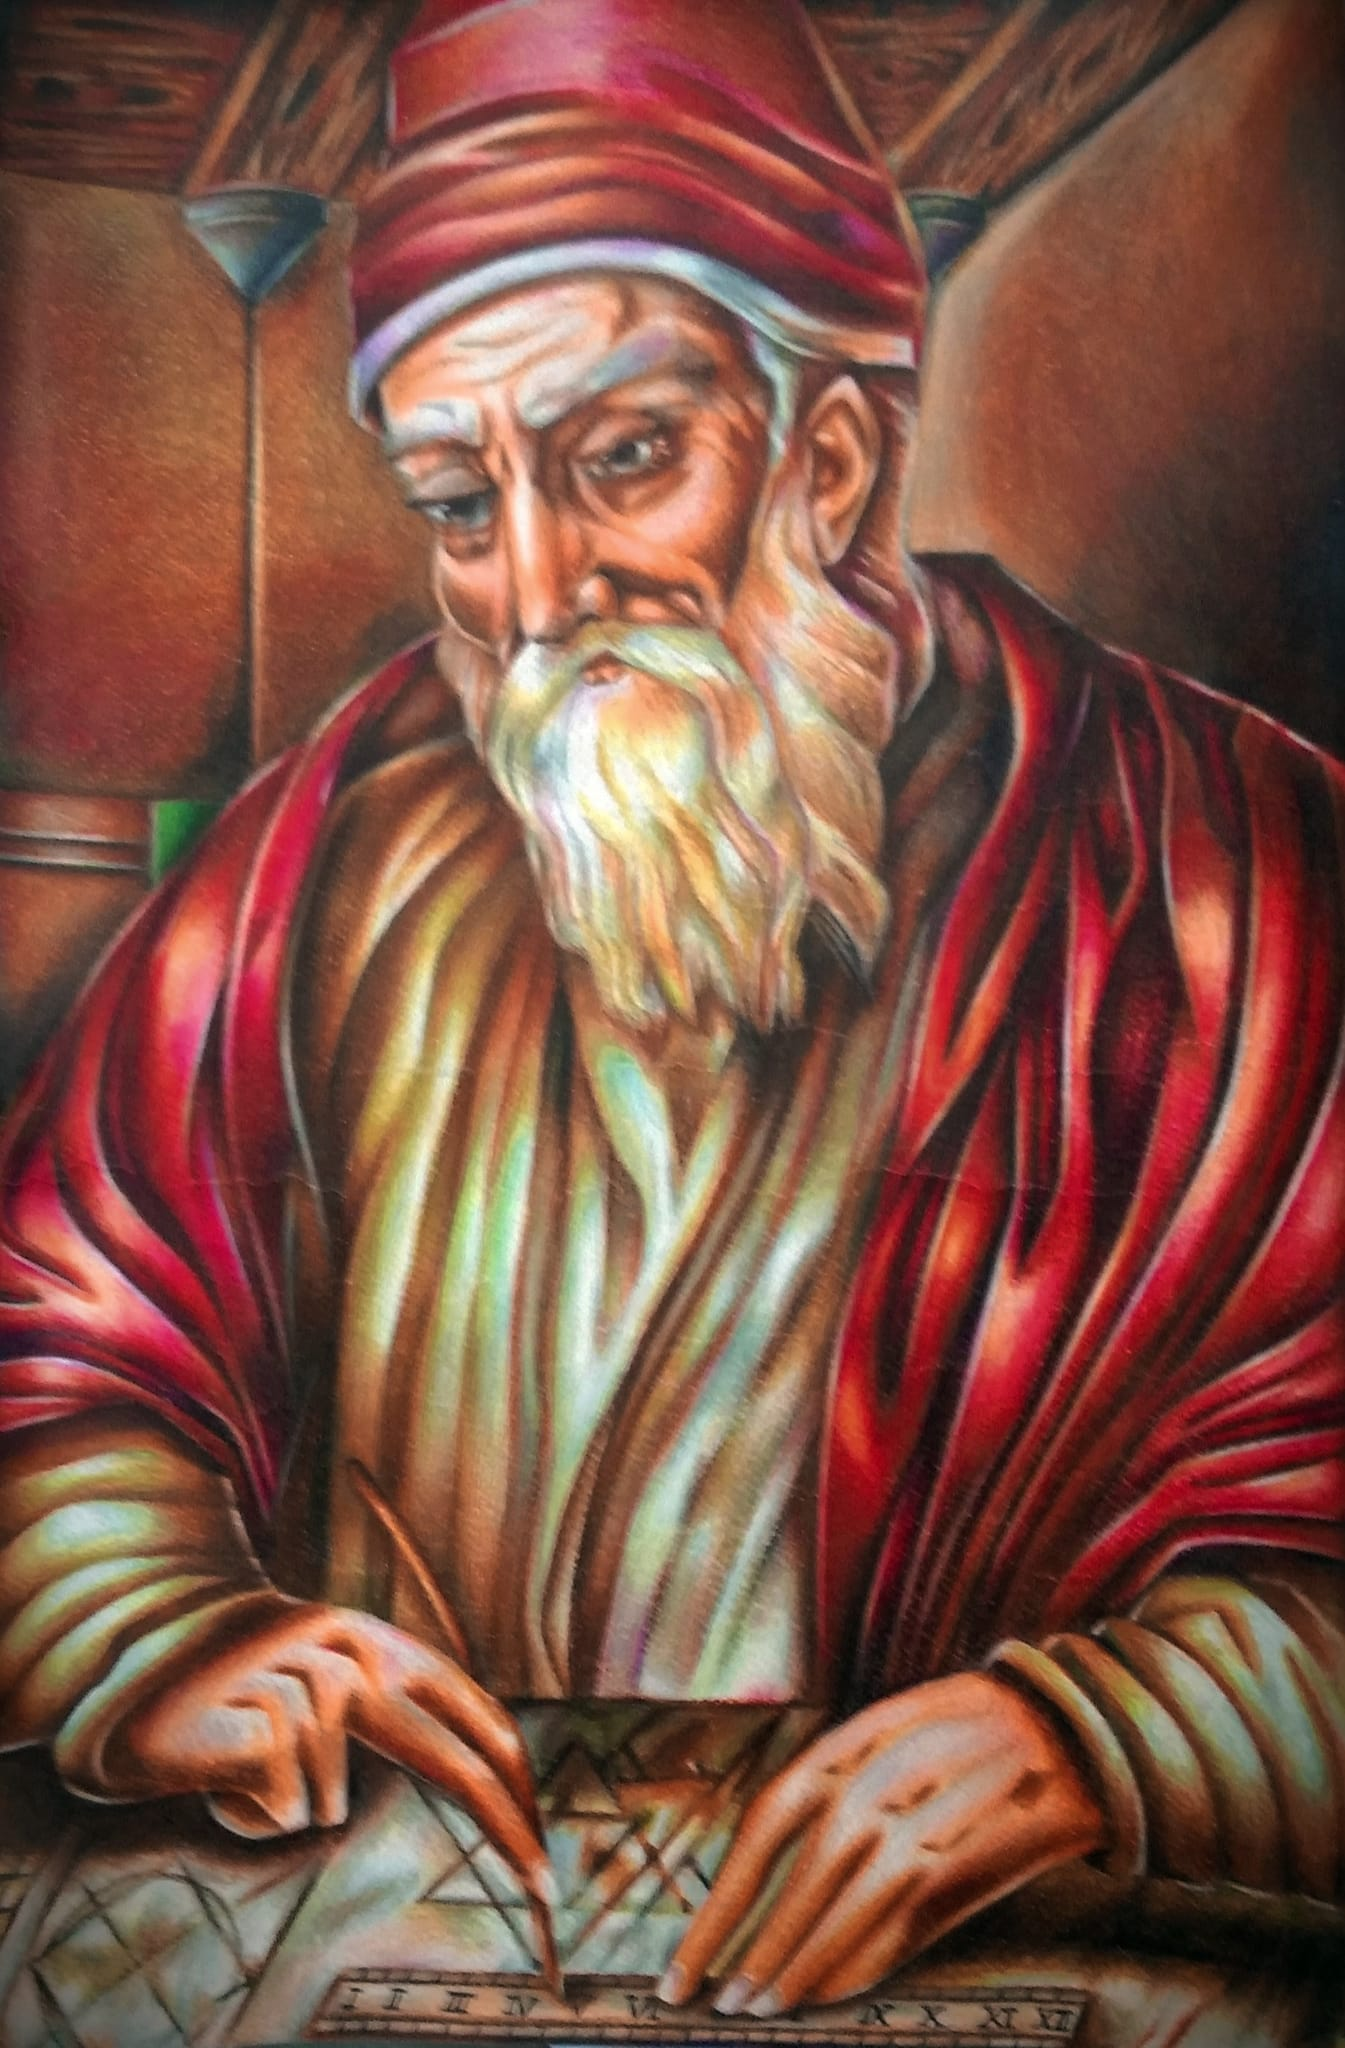
\includegraphics[width=0.7\textwidth]{images/euclid.jpg}
\\
\tiny Credit: Triphop Rattanajaratrod, CC BY-SA 3.0
\end{figure}
\end{column}
\end{columns}
\end{frame}

\begin{frame}{Euclid's Elements}
\begin{itemize}
\item 13 books
\item Used in teaching mathematics up until 19th century
\item Includes 5 postulates laying out the foundations of geometry
\end{itemize}
\end{frame}

\begin{frame}{Five Postulates of Euclidean Geometry}
\begin{enumerate}
\item A straight line segment may be drawn from any given point to any other.
\item A straight line may be extended to any finite length.
\item A circle may be described with any given point as its center and any distance as its radius.
\item All right angles are congruent.
\item If a straight line intersects two other straight lines, and so makes the two interior angles on one side of it
together less than two right angles, then the other straight lines will meet at a point if extended far enough on the
side on which the angles are less than two right angles.
\end{enumerate}
\end{frame}

\begin{frame}{Fifth Postulate Visualized}
\begin{figure}
\centering
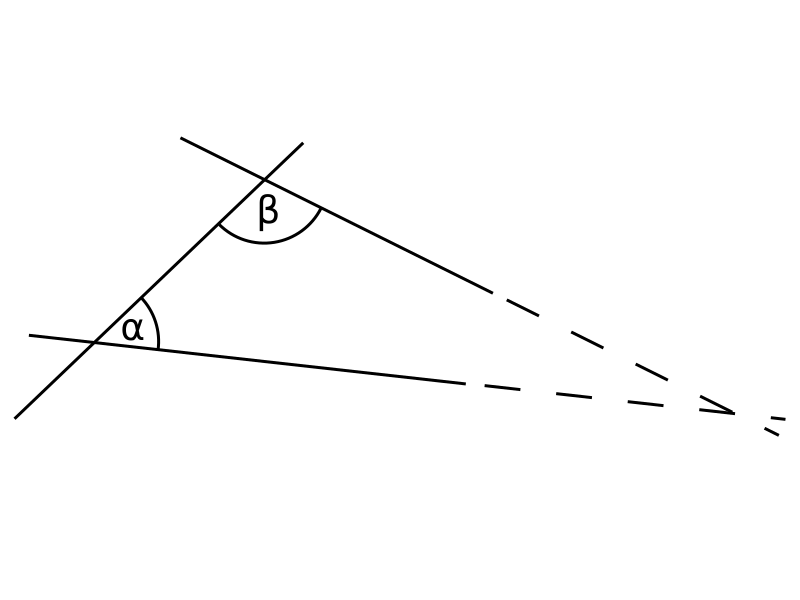
\includegraphics[width=0.7\textwidth]{images/fifth-postulate.png}
\\
\tiny Credit: Dickdock, CC BY-SA 3.0
\end{figure}
\end{frame}

\begin{frame}{The 5th Postulate}
\begin{itemize}
\item For centuries mathematicians consider the fifth postulate different from the other four
\item It is considered correct, but redundant
\item All attempts to formulate the fifth postulate in terms of the earlier four fail
\end{itemize}
\end{frame}

\begin{frame}{Giovanni Girolamo Saccheri (1667-1733)}
\begin{itemize}
\item Italian jesuit priest, born in 17th century
\item Attempts \emph{reductio ad absurdum}
\begin{itemize}
\item Assume the fifth postulate is incorrect
\item Should lead to inconsistencies and contradictions
\item No inconsistencies found
\end{itemize}
\end{itemize}
\end{frame}

\begin{frame}{After Saccheri}
\begin{itemize}
\item Gauss (1777-1855) is convinced a consistent geometry exists beyond Euclidean geometry
\item Farkas Bolayi (1775-1856) is Gauss' friend
\item Farkas spends a lot of his life attempting to discover a geometry beyond Euclidean geometry, but fails
\item J{\'a}nos Bolayi (1802-1860), son of Farkas, succeeds
\begin{itemize}
\item Appendix (1832)
\end{itemize}
\end{itemize}
\end{frame}

\begin{frame}{Nikolai Lobachevsky (1792-1856)}
\begin{columns}
\begin{column}{0.6\textwidth}
\begin{itemize}
\item Unbeknownst to J{\'a}nos Bolayi, Nikolai Lobachevsky managed to do it earlier
\begin{itemize}
\item Kasan Bulletin (1829–30)
\end{itemize}
\item Lobachevsky studied at Kazan University where Johann Christian Martin Bartels, a friend of Gauss, worked as a professor
\end{itemize}
\end{column}
\begin{column}{0.4\textwidth}
\begin{figure}
\centering
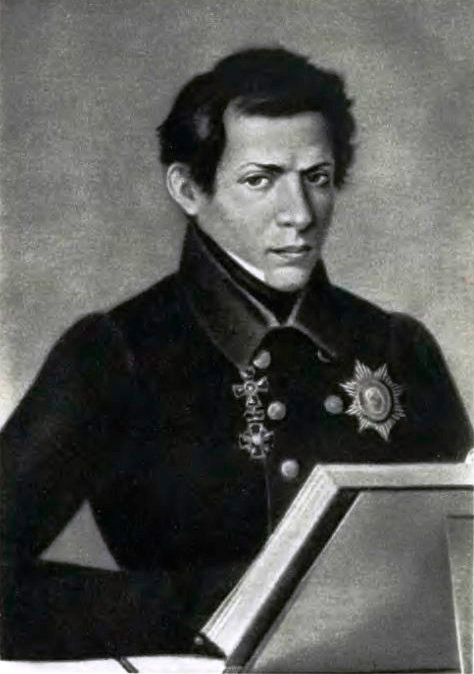
\includegraphics[width=0.8\textwidth]{images/lobachevsky.jpg}
\\
\tiny Credit: Lev Kriukov, public domain
\end{figure}
\end{column}
\end{columns}
\end{frame}

\part{Peano axioms}
\begin{frame}
\partpage
\end{frame}

\begin{frame}{Giuseppe Peano (1858 – 1932)}
\begin{columns}
\begin{column}{0.6\textwidth}
\begin{itemize}
\item Italian mathematician
\item Worked most of his career in University of Turin
\item Known for creating Peano Arithmetic
\end{itemize}
\end{column}
\begin{column}{0.4\textwidth}
\begin{figure}
\centering
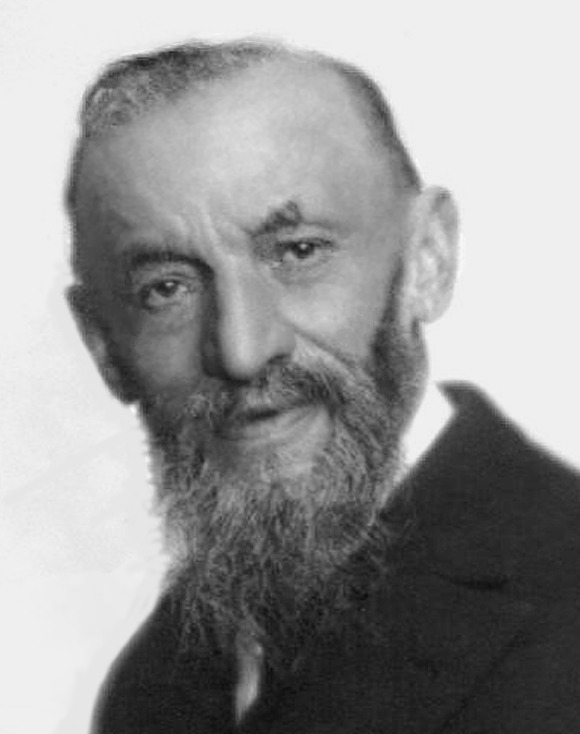
\includegraphics[width=0.8\textwidth]{images/peano.jpg}
\\
\tiny Credit: Unknown author, public domain
\end{figure}
\end{column}
\end{columns}
\end{frame}

\begin{frame}{Peano Arithmetic}
\begin{itemize}
\item Formal system for arithmetic and natural numbers
\item If you had to define the natural numbers, how would you do it..?
\end{itemize}
\end{frame}

\begin{frame}{Successor function}
\begin{itemize}
\item Decide that zero is a natural number
\item Define a successor function such that for each natural number, the successor function returns the next number,
which is also a natural number
\begin{itemize}
\item S0 = 1
\item S1 = 2
\item etc...
\end{itemize}
\item Successor function can be applied multiple times
\begin{itemize}
\item SS0 = 2
\item SSS0 = 3
\item etc...
\end{itemize}
\end{itemize}
\end{frame}

\begin{frame}{Peano Axioms}
\begin{itemize}
\item Zero is a natural number
\[ 0 \in \mathbb{N} \]
\item Zero is not the immediate successor of any natural number
\[ 0 \neq Sx \]
\item The immediate successor of any natural number is a natural number
\[ Sx \in \mathbb{N} \]
\end{itemize}
\end{frame}

\begin{frame}{More Peano Axioms}
\begin{itemize}
\item Natural numbers are
\begin{itemize}
\item Reflexive: each natural number is equal to itself
\[ x = x \]
\item Symmetric: if x and y are natural numbers and x = y, then y = x
\[ x = y \iff y = x \]
\item Transitive: if x = y and y = z then x = z
\[ (x = y \land y = z) \implies x = z \]
\end{itemize}
\end{itemize}
\end{frame}

\begin{frame}{Addition}
\begin{itemize}
\item a + 0 = a
\item a + 1 = Sa
\item a + 2 = SSa
\item ...
\item a + b = SSSS...SSa
\end{itemize}
\center{Apply the successor function b times!}
\end{frame}

\part{First-order logic}
\begin{frame}
\partpage
\end{frame}

\begin{frame}{Gottlob Frege (1848 – 1925)}
\begin{columns}
\begin{column}{0.6\textwidth}
\begin{itemize}
\item German philosopher, logician and mathematician
\item Studied at University of G{\"o}ttingen where he did his PhD
\item Frege wanted to create a formal language for all of mathematics
\end{itemize}
\end{column}
\begin{column}{0.4\textwidth}
\begin{figure}
\centering
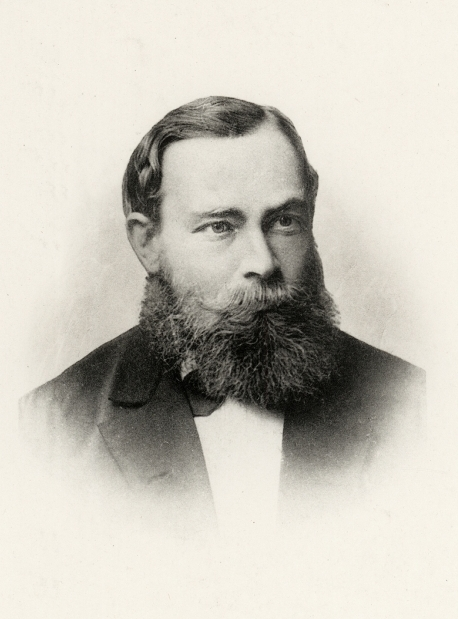
\includegraphics[width=0.8\textwidth]{images/frege.jpg}
\\
\tiny Credit: Unknown author, public domain
\end{figure}
\end{column}
\end{columns}
\end{frame}

\begin{frame}{Gottlob Frege cont.}
\begin{itemize}
\item Frege's goal was that everything in mathematics should be based on logic
\item No intuition involved
\item At the time, mathematics did not have a language for logic
\item Frege had to create it
\item Essentially, Frege created first-order logic, also known as predicate logic
\end{itemize}
\end{frame}

\begin{frame}{Propositional logic}
\begin{itemize}
\item Statements that have a truth value, i.e. they are either true or false
\item Example: "it rains or it doesn't"
\item Another example could be "it rains"
\end{itemize}
\end{frame}

\begin{frame}{Definition}
\begin{itemize}
\item Propositional logic has an alphabet consisting of
\begin{itemize}
\item proposition symbols: $x, y, z, ...$
\item connectives: $\land, \lor, \implies, \iff, \neg, \bot$
\item auxiliary symbols: $(, )$
\end{itemize}
\item Like any formal system, propositional logic uses predefined rules how to operate on statements
\end{itemize}
\end{frame}

\begin{frame}{Example}
\begin{itemize}
\item Let's define a proposition "it rains", i.e.:
\[ x := \text{"it rains"} \]
\item Now the proposition "it rains" is simply
\[ x \]
\item The proposition "it rains or it doesn't" is
\[ x \lor \neg x \]
\end{itemize}
\end{frame}

\begin{frame}{Example 2}
\begin{itemize}
\item Let's define propositions "it rains", "we have raincoats" and "we get wet"
\[ x := \text{"it rains"} \]
\[ y := \text{"we have raincoats"} \]
\[ z := \text{"we get wet"} \]
\item The statement from earlier, "if it rains and we don't have raincoats we get wet" can be stated as
\[ (x \land \neg y) \implies z \]
\end{itemize}
\end{frame}

\begin{frame}{Predicate logic}
\begin{itemize}
\item Propositional logic doesn't provide any means how to evaluate the propositions themselves
\item In predicate logic we use predicates for variables
\item Most importantly, we have quantifiers such as "for all" $\forall$ and "there exists" $\exists$
\end{itemize}
\end{frame}

\begin{frame}{Example}
\begin{itemize}
\item A proposition such as "x = 2y" doesn't mean much in itself
\item However, if we add a few quantifiers, it is more useful
\item "for all x, there is a y such that x = 2y"
\[ \forall x \exists y x = 2y \]
\end{itemize}
\end{frame}

\begin{frame}{Example 2}
\begin{itemize}
\item Can we give a definition for squares?
\[ \exists y x = y^2 \]
\item How about definition for primes?
\[ \forall a \forall b ab = x \implies a = 1 \lor b = 1 \]
\end{itemize}
\end{frame}

\part{Set Theory}
\begin{frame}
\partpage
\end{frame}

\begin{frame}{Georg Cantor (1845-1918)}
\begin{columns}
\begin{column}{0.6\textwidth}
\begin{itemize}
\item Born in St. Petersburg to Danish parents
\item His family moved to Frankfurt when he was just a child, in 1856
\item Cantor studied in University of G{\"o}ttingen and finished his PhD in 1867
\end{itemize}
\end{column}
\begin{column}{0.4\textwidth}
\begin{figure}
\centering
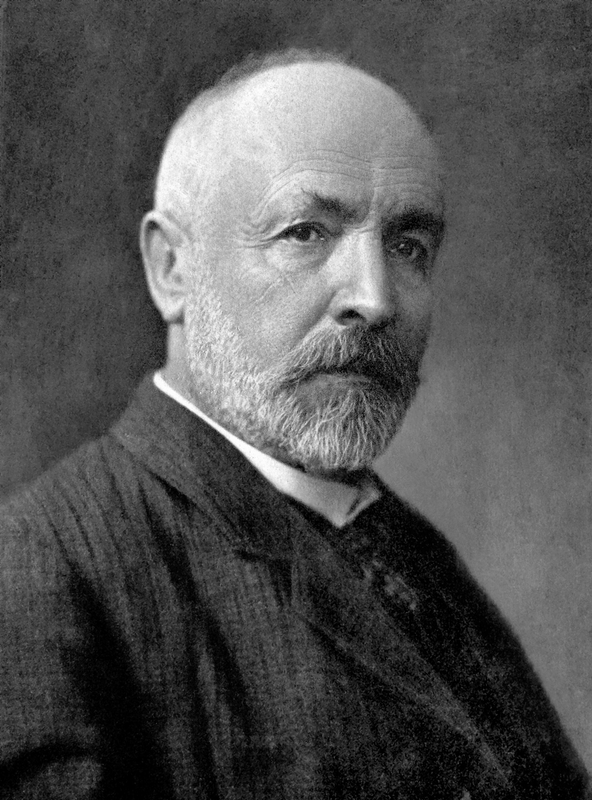
\includegraphics[width=0.8\textwidth]{images/cantor.png}
\\
\tiny Credit: Unknown author, public domain
\end{figure}
\end{column}
\end{columns}
\end{frame}

\begin{frame}{Georg Cantor (1845-1918)}
\begin{itemize}
\item Prior to Cantor, only "naive" set theory existed, i.e. set theory was limited to sets of finite size etc
\item Cantor revolutionized set theory by showing there are infinite sets of different size
\item Cantor showed that the amount of natural numbers, $\mathbb{N}$, is smaller than the amount of real numbers,
$\mathbb{R}$, between 0 and 1.
\end{itemize}
\end{frame}

\begin{frame}{Cantor's Diagonalization Argument}
\begin{itemize}
\item Enumerate all natural numbers, $\mathbb{N}$
\item For each natural number, pick a random real number, $\mathbb{R}$, that is bigger than 0 and smaller than 1, (0,
1), which is different from all the earlier
\item Create a new number by picking the digits from the "diagonal" and adding one, +1, to each digit (if the digit is
9, make it 8)
\item The new number is different from all the others
\end{itemize}
\end{frame}

\begin{frame}{Cantor's Diagonalization Argument}
\begin{center}
\begin{tabular}{| c | c |}
\hline
$\mathbb{N}$ & $\mathbb{R}$ \\
\hline
$1$ & $0.382149...$ \\
\hline
$2$ & $0.256348...$ \\
\hline
$3$ & $0.338852...$ \\
\hline
$4$ & $0.472019...$ \\
\hline
$5$ & $0.776221...$ \\
\hline
$6$ & $0.969832...$ \\
\hline
\end{tabular}
\end{center}
\end{frame}

\begin{frame}{Cantor's Diagonalization Argument}
\begin{center}
\begin{tabular}{| c | c |}
\hline
$\mathbb{N}$ & $\mathbb{R}$ \\
\hline
$1$ & $0.\textcolor{red}{3}82149...$ \\
\hline
$2$ & $0.2\textcolor{red}{5}6348...$ \\
\hline
$3$ & $0.33\textcolor{red}{8}852...$ \\
\hline
$4$ & $0.472\textcolor{red}{0}19...$ \\
\hline
$5$ & $0.7762\textcolor{red}{2}1...$ \\
\hline
$6$ & $0.96983\textcolor{red}{2}...$ \\
\hline
\end{tabular}
\end{center}
\end{frame}

\begin{frame}{Cantor's Diagonalization Argument}
\begin{center}
\begin{tabular}{| c | c |}
\hline
$\mathbb{N}$ & $\mathbb{R}$ \\
\hline
$1$ & $0.\textcolor{red}{3}82149...$ \\
\hline
$2$ & $0.2\textcolor{red}{5}6348...$ \\
\hline
$3$ & $0.33\textcolor{red}{8}852...$ \\
\hline
$4$ & $0.472\textcolor{red}{0}19...$ \\
\hline
$5$ & $0.7762\textcolor{red}{2}1...$ \\
\hline
$6$ & $0.96983\textcolor{red}{2}...$ \\
\hline
& $\textcolor{red}{0.469133...}$ \\
\hline
\end{tabular}
\end{center}
\end{frame}

\part{Russell's Paradox}
\begin{frame}
\partpage
\end{frame}

\begin{frame}{Bertrand Russell (1872-1970)}
\begin{columns}
\begin{column}{0.6\textwidth}
\begin{itemize}
\item British mathematician and politician
\item His grandfather was twice the prime minister of the United Kingdom
\item Bertrand Russell's first publication was on German Social Democracy (1896)
\end{itemize}
\end{column}
\begin{column}{0.4\textwidth}
\begin{figure}
\centering
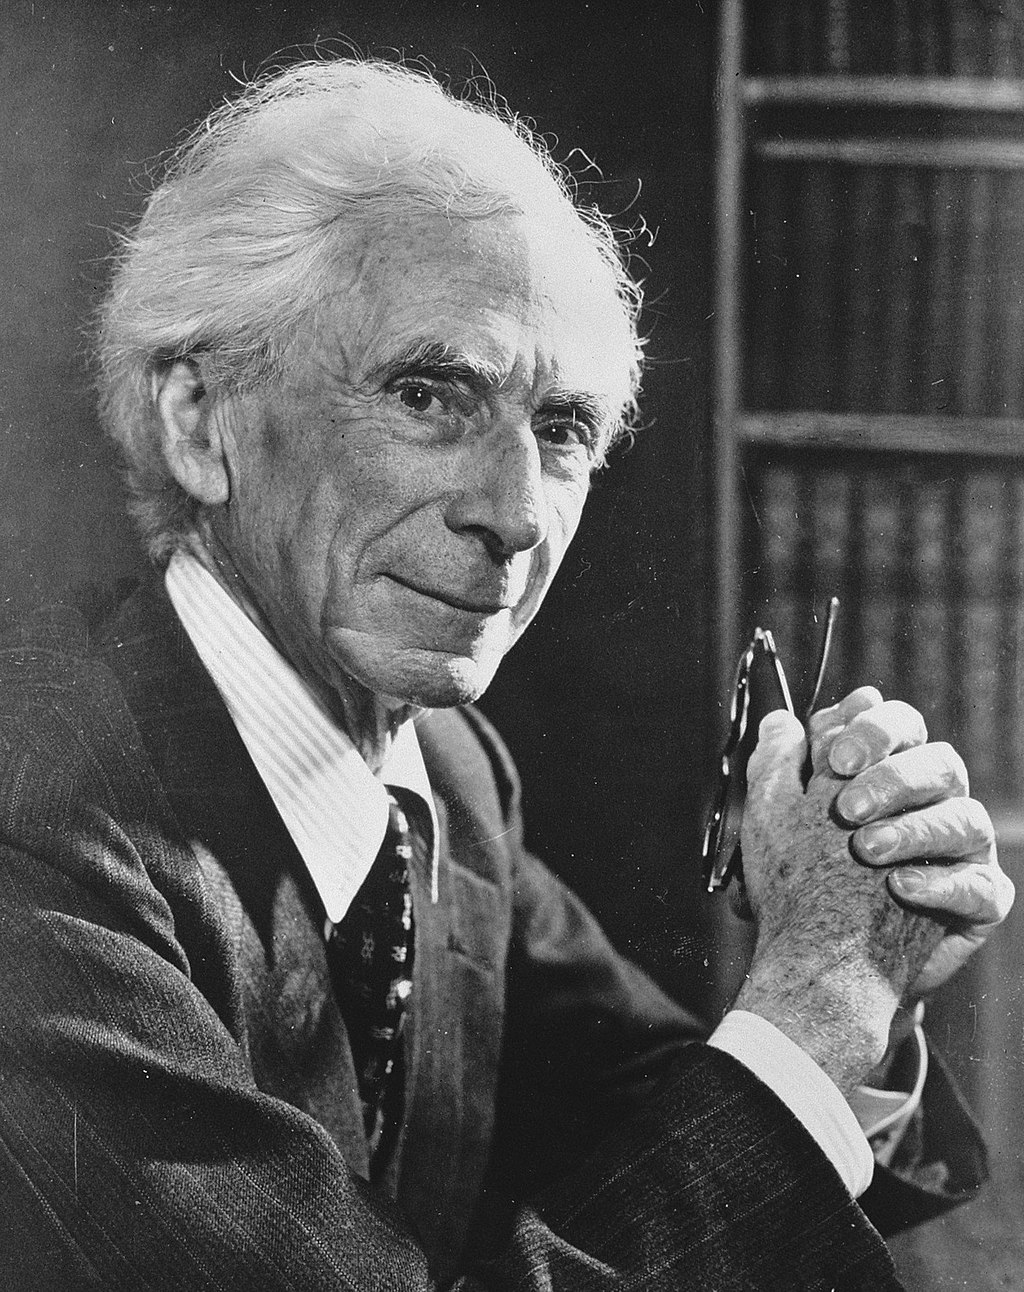
\includegraphics[width=0.8\textwidth]{images/russell.jpg}
\\
\tiny Credit: Anefo, CC0
\end{figure}
\end{column}
\end{columns}
\end{frame}

\begin{frame}{Set Theory and Peano}
\begin{itemize}
\item Bertrand Russell meets Giuseppe Peano and other influential Italian mathematicians in a Congress in Paris in 1900
\item This sparks Russell's interest in Set Theory
\item Russell discovers Russell's Paradox
\item Exact year is unknown, most likely 1901
\item The Principles of Mathematics (1903) is a book by Russell where he presents the paradox
\end{itemize}
\end{frame}

\begin{frame}{Russell's Paradox (Layman version)}
\begin{itemize}
\item There is a small town with exactly one barber
\begin{itemize}
\item The barber shaves every man who does not shave himself
\item The barber does not shave men who shave themselves
\item Should the barber shave himself?
\end{itemize}
\item If the barber shaves himself, he should not
\item If the barber does not shave himself, he should
\end{itemize}
\end{frame}

\begin{frame}{Russell's Paradox (Formal version)}
\begin{itemize}
\item The set of all sets that do not contain themselves
\item Should this set contain itself?
\item If it contains itself, it should not
\item If it doesn't, it should
\end{itemize}
\end{frame}

\part{Hilbert's Program}
\begin{frame}
\partpage
\end{frame}

\begin{frame}{David Hilbert (1862-1943)}
\begin{columns}
\begin{column}{0.6\textwidth}
\begin{itemize}
\item Studied, did his PhD and worked at University of K{\o}nigsberg
\item 1895: became a professor at University of G{\"o}ttingen
\end{itemize}
\end{column}
\begin{column}{0.4\textwidth}
\begin{figure}
\centering
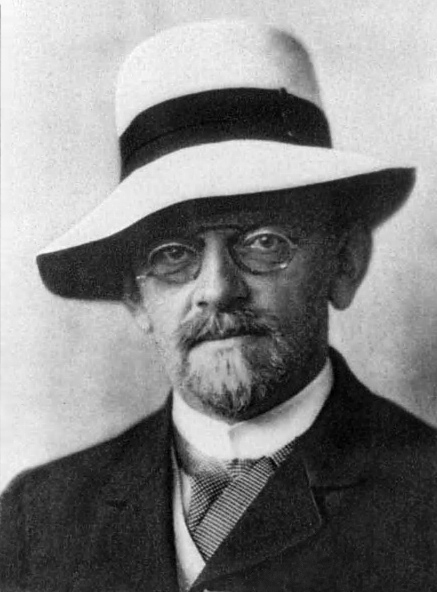
\includegraphics[width=0.8\textwidth]{images/hilbert.jpg}
\\
\tiny Credit: Unknown author, public domain
\end{figure}
\end{column}
\end{columns}
\end{frame}

\begin{frame}{Axiomatization of geometry}
\begin{itemize}
\item In 1899 Hilbert publishes his axiomatization of geometry
\item Grundlagen der Geometrie
\item Foundations of Geometry
\item To avoid weaknesses in previous attempts by others, Hilbert does not use terms such as "points" and "lines", but
talks about abstract objects such as "shoes" and "tables"
\end{itemize}
\end{frame}

\begin{frame}{Formalism vs Intuitionism}
\begin{itemize}
\item Cantor's diagonalization argument was not well accepted by everyone
\item Leopold Kronecker: Cantor is a "scientific charlatan" and "corrupter of youth"
\item L. E. J. Brouwer founded the mathematical school of thought known as intuitionism
\item Brouwer was not convinced that every statement in logic would be either true or false and published a paper on the "law of the excluded middle"
\item Emil du Bois-Reymond: ignoramus et ignorabimus (we do not know and will not know)
\end{itemize}
\end{frame}

\begin{frame}{Hilbert's Response}
\begin{itemize}
\item Hilbert was already know by his rigorous use of axioms and thus, formalism
\item Hilbert: Wir müssen wissen. Wir werden wissen.
\item We must know. We will know.
\item Hilbert: Aus dem Paradies, das Cantor uns geschaffen, soll uns niemand vertreiben k{\"o}nnen
\item From the paradise, that Cantor created for us, no-one shall be able to expel us.
\end{itemize}
\end{frame}

\begin{frame}{Ignoramus}
\begin{columns}
\begin{column}{0.6\textwidth}
\begin{itemize}
\item Ignoramus et ignorabimus
\begin{itemize}
\item Wir müssen wissen. Wir werden wissen.
\end{itemize}
\item We cannot know and we will not know
\begin{itemize}
\item We must know. We will know.
\end{itemize}
\item Hilbert's response is inscribed on his tomb
\end{itemize}
\end{column}
\begin{column}{0.4\textwidth}
\begin{figure}
\centering
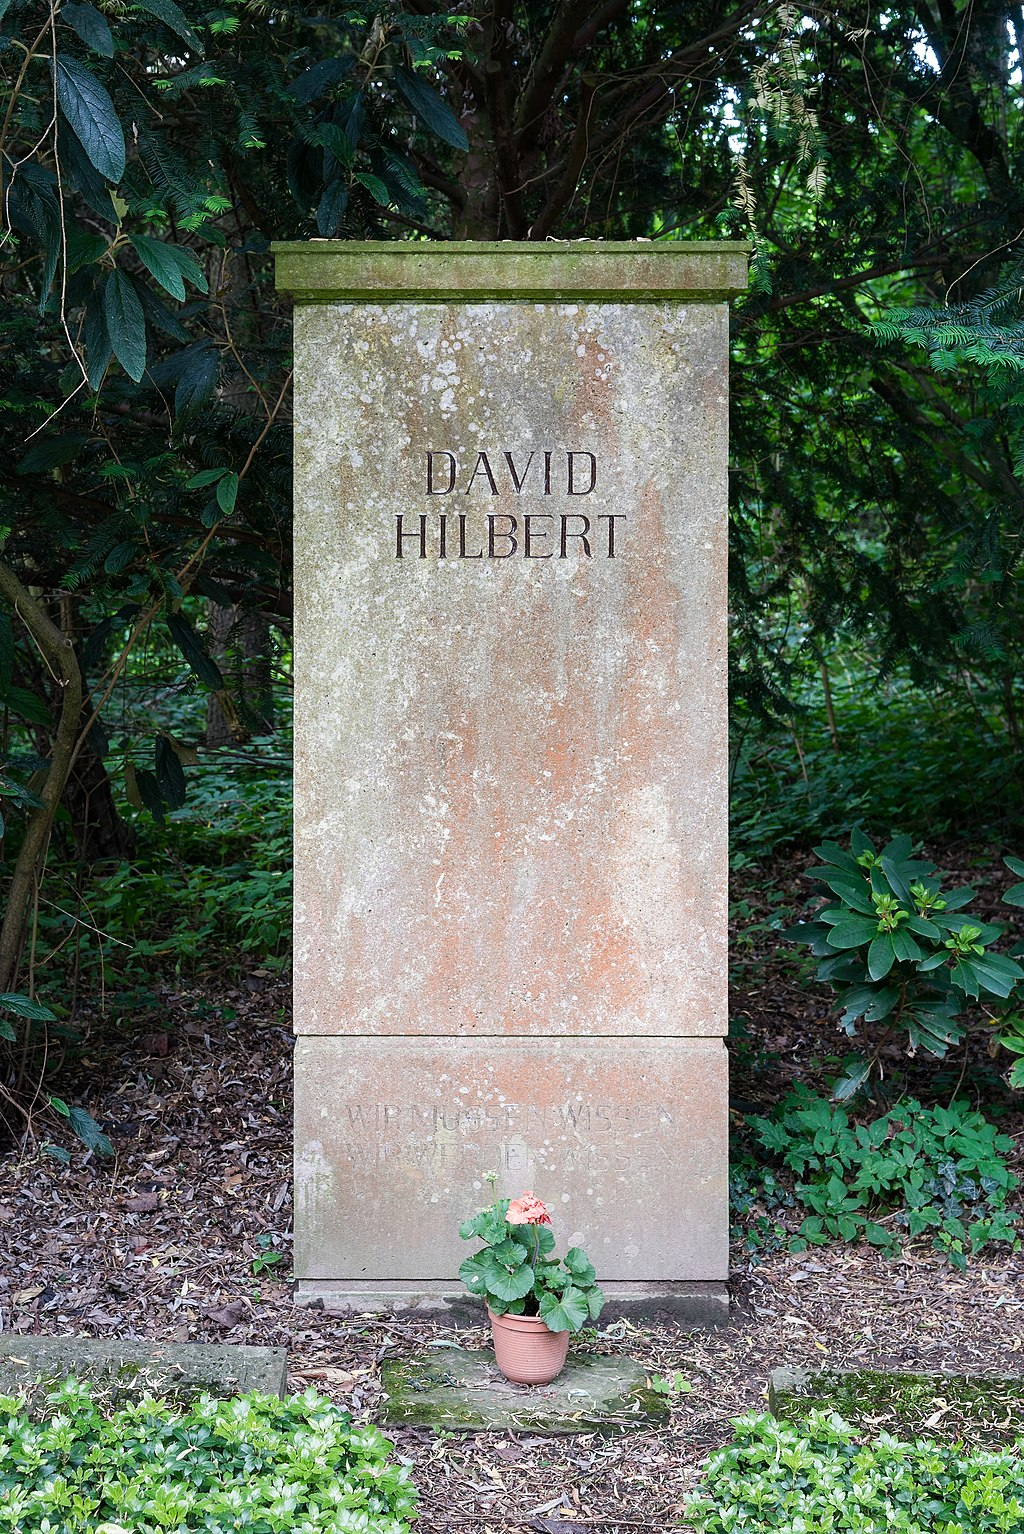
\includegraphics[width=0.8\textwidth]{images/hilbert-tomb.jpg}
\\
\tiny Credit: Julian Herzog, CC BY 4.0
\end{figure}
\end{column}
\end{columns}
\end{frame}

\begin{frame}{Hilbert's Program}
\begin{itemize}
\item Create a formal system for all of mathematics
\item The formal system must fulfill the following criteria:
\begin{itemize}
\item Completeness: Every true statement must be provable within the system
\item Consistency: No inconsistencies must exist in the system
\item Decidability: There must exist an effective procedure to determine whether each statement is true of false
\end{itemize}
\end{itemize}
\end{frame}

\part{Principia Mathematica}
\begin{frame}
\partpage
\end{frame}

\begin{frame}{Principia Mathematica}
\begin{itemize}
\item Authored by Bertrand Russell and Alfred North Whitehead
\item 3 volumes published in 1910-1913
\end{itemize}
\end{frame}

\begin{frame}{Goal}
\begin{itemize}
\item Russell and Whitehead wanted to create formal system for all of mathematics
\item The system they created is based on logic and set theory
\item While they borrowed many ideas from Frege, they wanted to create a system free of contradictions
\end{itemize}
\end{frame}

\begin{frame}{Theory of Types}
\begin{itemize}
\item To avoid Russell's Paradox, Principia Mathematica introduces a "Theory of Types"
\item A set can contain only elements of types that are lower in hierarchy
\item "The set of all sets that do not include themselves" is in violation of the theory of types
\end{itemize}
\end{frame}

\part{G{\"o}del's Incompleteness Theorem}
\begin{frame}
\partpage
\end{frame}

\begin{frame}{Kurt G{\"o}del (1906-1978)}
\begin{columns}
\begin{column}{0.6\textwidth}
\begin{itemize}
\item Austro-Hungarian Mathematician
\item Finished his PhD in 1930, which was about first-order logic
\item His PhD was likely motivated by Hilbert's Program
\end{itemize}
\end{column}
\begin{column}{0.4\textwidth}
\begin{figure}
\centering
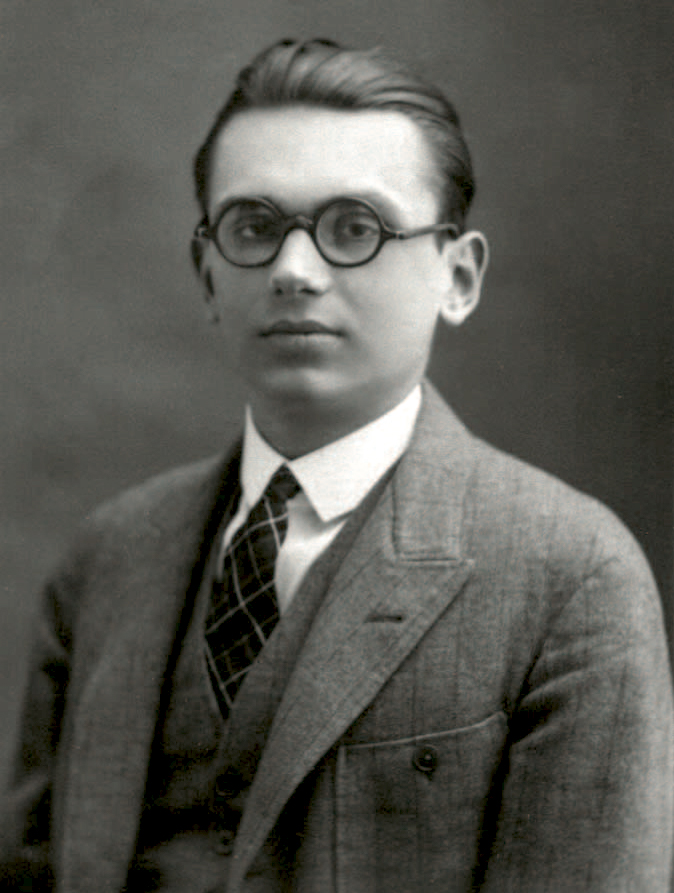
\includegraphics[width=0.8\textwidth]{images/goedel.jpg}
\\
\tiny Credit: Unknown author, public domain
\end{figure}
\end{column}
\end{columns}
\end{frame}

\begin{frame}{Conference in K{\"o}nigsberg}
\begin{itemize}
\item Held on 5–7 September 1930
\item One of the main tracks was about the foundations of mathematics
\item Among presenters were G{\"o}del and von Neumann
\item This conference is the first place where G{\"o}del hinted at the incompleteness of mathematics
\item Several sources state John von Neumann was the only one who understood the implications and pulled G{\"o}del
aside to talk about it more
\end{itemize}
\end{frame}

\begin{frame}{G{\"o}del paper}
\begin{itemize}
\item {\"U}ber formal unentscheidbare S{\"a}tze der Principia Mathematica und verwandter Systeme I
\item On Formally Undecidable Propositions of Principia Mathematica and Related Systems I
\item Submitted November 17, 1930
\item Published in 1931
\end{itemize}
\end{frame}

\begin{frame}{G{\"o}del Numbering}
\begin{itemize}
\item G{\"o}del created a numbering scheme where every statement in predicate logic has a number
\item 1. Create an alphabet of all the symbols in the formal system
\item 2. Assign a number $x$ to each symbol
\item 3. Use prime numbers $y$ to indicate the position of each symbol in a statement
\item 4. Replace the symbols with $y^x$
\item 5. Multiply the symbols together to figure out the unique number of the statement
\end{itemize}
\begin{center}
Note: the original statement can be reconstructed using prime factorization!
\end{center}
\end{frame}

\begin{frame}{Example}
\begin{itemize}
\item Alphabet:
\[ \forall - 1, \exists - 2, = - 3, x - 4, y - 5 \]
\item Sentence:
\[ \forall x \exists y x = y \]
\item G{\"o}del numbering:
\[ 2^\forall 3^x 5^\exists 7^y 11^x 13^= 17^y \]
\[ 2^1 3^4 5^2 7^5 11^4 13^3 17^5 \]
\[ 3108784570194441288150 \]
\end{itemize}
\end{frame}

\begin{frame}{Example with successor function}
\begin{itemize}
\item G{\"o}del numbering uses the successor function to define numerals
\item If we want to say $x = 5$, our statement is: $x = SSSSS0$
\item Alphabet: $x - 1$, $= - 2$, $S - 3$, $0 - 4$
\item Statement G{\"o}del number:
\[ 2^1 3^2 5^3 7^3 11^3 13^3 17^3 19^4\]
\[ 1444927040236093664250 \]
\end{itemize}
\end{frame}

\begin{frame}{Fixpoint theorem}
\begin{itemize}
\item For every function with one free variable, we can create a G{\"o}del number g such that
\[ G \iff F(g) \]
\item This is also known as the diagonal lemma
\item The fixpoint theorem allows us to create statements that speak of themselves
\end{itemize}
\end{frame}

\begin{frame}{G{\"o}del's First Incompleteness Theorem}
\begin{itemize}
\item There are valid statements that are not provable, i.e. have no proof
\item "This statement is not provable"
\[ G \iff \neg Prov(g) \]
\end{itemize}
\end{frame}

\begin{frame}{Axioms}
\begin{itemize}
\item Axioms have no proof, they just are
\item We can create formal system F' which is an extension of formal system F where a non-provable statement is added
as an axiom
\item Is F' complete?
\item No, because there's an infinite amount of non-provable statements
\end{itemize}
\end{frame}

\begin{frame}{G{\"o}del's Second Incompleteness Theorem}
\begin{itemize}
\item Let's create a statement that defines the consistency of the formal system F
\[ Cons(F) \]
\item G{\"o}del showed that this statement cannot be proved within itself
\end{itemize}
\end{frame}

\part{The von Neumann Architecture}
\begin{frame}
\partpage
\end{frame}

\begin{frame}{John von Neumann (1903-1957)}
\begin{columns}
\begin{column}{0.6\textwidth}
\begin{itemize}
\item Born Neumann J{\'a}nos Lajos
\item Hungarian mathematician
\item Did his PhD on axiomatization of Cantor's Set Theory
\item As a post-doc, moved to University of G{\"o}ttingen to study under Hilbert
\end{itemize}
\end{column}
\begin{column}{0.4\textwidth}
\begin{figure}
\centering
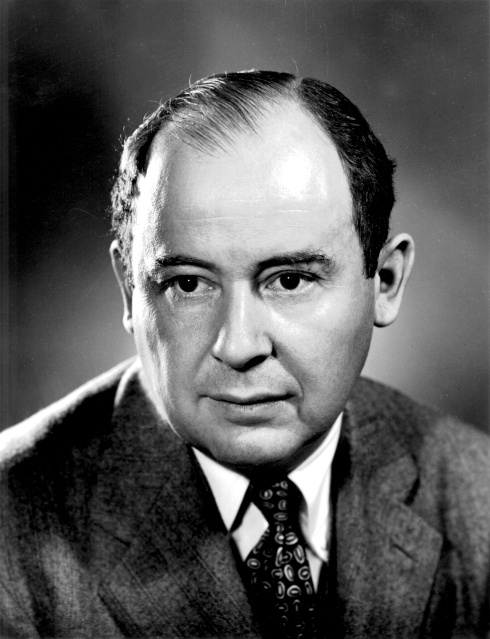
\includegraphics[width=0.8\textwidth]{images/vonneumann.jpg}
\\
\tiny Credit: Los Alamos National Laboratory, Attribution
\end{figure}
\end{column}
\end{columns}
\end{frame}

\begin{frame}{The ENIAC}
\begin{itemize}
\item Electronic Numerical Integrator And Computer
\item Built between 1943-45
\item The first general-purpose computer
\end{itemize}
\end{frame}

\begin{frame}{Programming the ENIAC}
\begin{itemize}
\item The ENIAC was fully electronic, i.e. it did not use any mechanical parts etc
\item However, the algorithm the ENIAC would run was determined by plugboards
\item In other words, if operators wanted to change the algorithm, they had to take the ENIAC offline and rewire the
plugboards
\end{itemize}
\end{frame}

\begin{frame}{The EDVAC report}
\begin{itemize}
\item Electronic Discrete Variable Automatic Computer
\item An unfinished 101-page report written by John von Neumann in 1945
\item Full title: First Draft of a Report on the EDVAC
\end{itemize}
\end{frame}

\begin{frame}{McCulloch-Pitts Neuron}
\begin{itemize}
\item The EDVAC report does not discuss vacuum tubes, but "idealized neurons"
\item von Neumann and other contemporaries wanted to build "electronic brains"
\item The only reference in the EDVAC report is to an article by neurophysiologist Warren McCulloch and mathematician Walter
Pitts
\end{itemize}
\end{frame}

\begin{frame}{McCulloch-Pitts Neuron cont.}
\begin{itemize}
\item A logical calculus of the ideas immanent in nervous activity (1943)
\item The paper describes a way to simulate a simplified version of a neuron
\item Using networks of these neurons, it is possible to learn, calculate, store data and execute logical functions
\end{itemize}
\end{frame}

\begin{frame}{EDVAC's Five "Organs"}
\begin{itemize}
\item Central arithmetic: performs mathematical operations such as addition and multiplication
\item Central control: ordering of instructions
\item Memory: stores computer code and numbers
\item Input: How to feed input to the computer
\item Output: How to retrieve output from the computer
\end{itemize}
\end{frame}

\begin{frame}{Programming the EDVAC}
\begin{itemize}
\item von Neumann was very familiar with G{\"o}del numbering
\item The same idea is used to program the EDVAC
\item Instructions are just "numbers"
\end{itemize}
\end{frame}

\begin{frame}{Self-reference}
\begin{itemize}
\item Does this mean we have self-reference?
\item Yes!
\item How else would you have programs that compile and run programs..?
\end{itemize}
\end{frame}

\part{Key Takeaways}
\begin{frame}
\partpage
\end{frame}

\begin{frame}{Everything is Set Theory}
\begin{itemize}
\item Everything in Computer Science is Set Theory
\item We have sets of data and we want to do set operations on them
\item This is why map, filter and fold are so essential for all programming
\end{itemize}
\end{frame}

\begin{frame}{LISP is awesome!}
\begin{itemize}
\item LISP is based on a very solid mathematical foundation
\item Lambda Calculus
\item Hence, LISP will never become obsolete
\end{itemize}
\end{frame}

\begin{frame}{When designing a programming language}
\begin{itemize}
\item The mathematical groundwork matters when designing a programming language
\item For instance, why does the industry keep on inventing countless configuration languages?
\end{itemize}
\end{frame}

\part{Extra}
\begin{frame}
\partpage
\end{frame}

\begin{frame}{The first computer program}
\begin{itemize}
\item The first computer program ever was a Monte Carlo Simulation
\item Prior to this, Monte Carlo Simulation did not exist
\item Why would it.. it was not feasible before fast computers!
\end{itemize}
\end{frame}

\begin{frame}{Monte Carlo Simulation}
\begin{itemize}
\item You know all possible outcomes and their probabilities, respectively
\item But there are too many scenarios, not feasible to solve analytically
\item In Monte Carlo Simulation, you run a simulation over and over again in order to retrieve the distribution of
likelihoods of outcomes
\end{itemize}
\end{frame}

\begin{frame}{The first Random Number Generator}
\begin{itemize}
\item Monte Carlo Simulation requires a Random Number Generator (RNG)
\item Random Number Generator did not exist (why they have?)
\item John von Neumann had to create one
\end{itemize}
\end{frame}

\begin{frame}{Middle-Square Method}
\begin{itemize}
\item Presented by John von Neumann in 1949
\item Start with a number that has n bits
\item Square the number
\item The new number has 2n bits
\item Use the middle bits
\item Those bits are the new "random" number
\item Use the number as input to create the next "random" number
\end{itemize}
\end{frame}

\begin{frame}[fragile]
\frametitle{Pseudocode}
\begin{verbatim}
a = 0xDEADBEEF
b = a^2
c = b[16:48]
a = c
\end{verbatim}
\end{frame}

\end{document}
